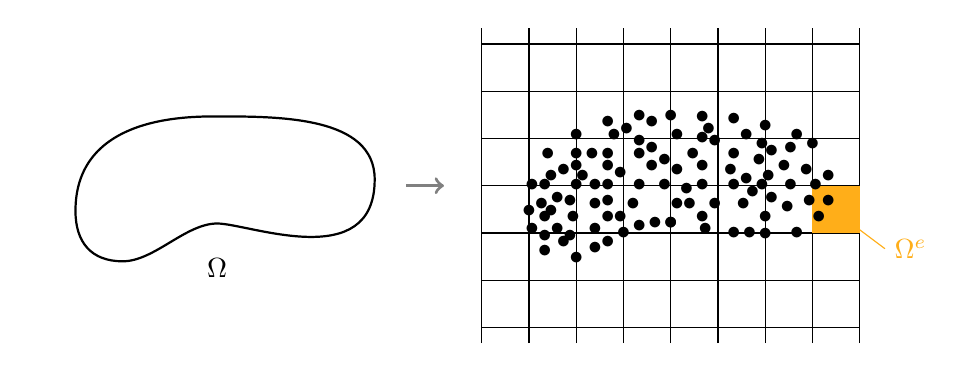
\begin{tikzpicture}[scale=0.8]
  \draw[white] (-3,-1) -- (3,-1) -- (3,4) -- (-3,4) -- (-3,-1);
  \begin{scope}[scale=0.5]
    \draw[thick] (-3,0.6) .. controls +(1,0) and +(-1,0) .. (0,1.8)  
    .. controls +(1,0) and +(0,-3) .. (5,3.2) 
    .. controls +(0,2) and +(2,0)  .. (0,5.2) 
    .. controls +(-1,0) and +(0,3) .. (-4.5,2.2) 
    .. controls +(0,-1) and +(-1,0).. (-3,0.6) ;
    \begin{scope}  % pour limiter la portée du clip
      \clip (-3,0.6) .. controls +(1,0) and +(-1,0) .. (0,1.8) 
      .. controls +(1,0) and +(0,-3) .. (5,3.2)
      .. controls +(0,2) and +(2,0)  .. (0,5.2)
      .. controls +(-1,0) and +(0,3) .. (-4.5,2.2)
      .. controls +(0,-1) and +(-1,0).. (-3,0.6);
    \end{scope}
    \node[below] at (0,1) {$\Omega$};
  \end{scope}
  \draw [->,very thick,gray] (3.,1.5) -- (3.6,1.5);
  \begin{scope}[xshift=7.2 cm]
    \draw[step=.75,black,thin] (-3.,-1.) grid (3,4.);
    % \draw[line width=0.6mm,Red] (-2.25,2.25) -- (-2.25,2.25)-- (-2.25,3)-- (2.25,3) --(2.25,2.25) -- (3.,2.25)-- (3.,0.75) --(2.25,0.75) --(2.25,0.) -- (0.75,0.) --(0.75,0.75) --(-0.75,0.75)-- (-0.75,0.)-- (-2.25,0.) -- (-2.25,0.75) --  (-3.,0.75)--(-3.,1.5) --(-2.25,1.5)--(-2.25,2.25);
    \fill[Orange!90,opacity=1] (2.25,.75) rectangle (3.,1.5);
    \draw[Orange!90] (2.6,1.1) -- (3.4,0.5) node [right]  {$\Omega^e$};

    % contour
    \node at (0,0.9) {$\bullet$}  ; \node at (2.5,1.65) {$\bullet$}  ; 
    \node at (0,2.6) {$\bullet$}  ;\node at (-2.25,1.1) {$\bullet$}  ; 
    \node at (-1.5,0.35) {$\bullet$}  ; \node at (-2.,0.45) {$\bullet$}  ;
    \node at (-2.2,1.5) {$\bullet$}  ; \node at (-1.5,2.3) {$\bullet$}  ; 
    \node at (2.35,1.) {$\bullet$}  ; \node at (2.25,2.15) {$\bullet$}  ;
    \node at (0.55,0.8) {$\bullet$}  ; \node at (-0.5,2.6) {$\bullet$}  ; 
    \node at (0.5,2.59) {$\bullet$}  ; \node at (1.5,2.45) {$\bullet$}  ;
    \node at (1,0.75) {$\bullet$}; \node at (2,0.75) {$\bullet$}  ;
    \node at (2,2.3) {$\bullet$}  ; \node at (1,2.55) {$\bullet$}  ;
    \node at (-1,2.5) {$\bullet$}  ; \node at (-1.95,2.) {$\bullet$}  ;
    % interior
    \node at (-1.5,1.5) {$\bullet$}  ; \node at (-1.25,2.) {$\bullet$}  ;
    \node at (-0.75,0.75) {$\bullet$}  ; \node at (-1.55,1.) {$\bullet$}  ;
    \node at (-0.5,1.5) {$\bullet$}  ; \node at (-0.5,2.) {$\bullet$}  ;
    \node at (0.25,1.45) {$\bullet$}  ; \node at (0.35,2.) {$\bullet$}  ;
    \node at (0.95,1.75) {$\bullet$}  ; \node at (1.15,1.2) {$\bullet$}  ;
    \node at (1.45,2.15) {$\bullet$}  ; \node at (1.55,1.65) {$\bullet$}  ;
    \node at (1.85,1.15) {$\bullet$}  ; \node at (2.15,1.75) {$\bullet$}  ;
    \node at (-1.,1.25) {$\bullet$}  ;
    \node at (-1.,1.5) {$\bullet$}  ; \node at (-1.2,1.2) {$\bullet$}  ;
    \node at (-1.,1.) {$\bullet$}  ; \node at (-1.2,0.8) {$\bullet$}  ;
    \node at (-2.,.7) {$\bullet$}  ; \node at (-1.8,0.8) {$\bullet$}  ;
    \node at (-1.7,.6) {$\bullet$}  ; \node at (-1.6,0.7) {$\bullet$}  ;
    \node at (-2.2,.8) {$\bullet$}  ; \node at (-2.,1.) {$\bullet$}  ;
    \node at (-2.05,1.2) {$\bullet$}  ; \node at (-1.9,1.1) {$\bullet$}  ;
    \node at (-2.0,1.5) {$\bullet$}  ; \node at (-1.9,1.65) {$\bullet$}  ;
    \node at (-1.8,1.3) {$\bullet$}  ; \node at (-1.6,1.25) {$\bullet$}  ;
    \node at (-1.7,1.75) {$\bullet$}  ; \node at (-1.5,1.8) {$\bullet$}  ;
    \node at (-1.4,1.65) {$\bullet$}  ; \node at (-1.2,1.5) {$\bullet$}  ;
    \node at (-1.,0.6) {$\bullet$}  ; \node at (-1.2,0.5) {$\bullet$}  ;
    \node at (-0.5,0.85) {$\bullet$}  ; \node at (-.25,0.9) {$\bullet$}  ;
    \node at (1.25,0.75) {$\bullet$}  ; \node at (1.5,0.72) {$\bullet$}  ;
    \node at (-.8,1.) {$\bullet$}  ; \node at (-.6,1.2) {$\bullet$}  ;
    \node at (.5,1.) {$\bullet$}  ; \node at (.7,1.2) {$\bullet$}  ;
    \node at (1.5,1.) {$\bullet$}  ; \node at (.3,1.2) {$\bullet$}  ;
    \node at (0.,.9) {$\bullet$}  ; \node at (.1,1.2) {$\bullet$}  ;
    \node at (-0.1,1.9) {$\bullet$}  ; \node at (.1,2.3) {$\bullet$}  ;
    \node at (0.1,1.75) {$\bullet$}  ; \node at (-.1,1.5) {$\bullet$}  ;
    \node at (-1.5,2) {$\bullet$}  ; \node at (-1.,1.8) {$\bullet$}  ;
    \node at (-1.,2) {$\bullet$}  ; \node at (-.9,2.3) {$\bullet$}  ;
    \node at (-.8,1.7) {$\bullet$}  ; \node at (-.5,2.2) {$\bullet$}  ;
    \node at (-0.7,2.4) {$\bullet$}  ; \node at (-.3,2.1) {$\bullet$}  ;
    \node at (-.3,2.5) {$\bullet$}  ; \node at (-.3,1.8) {$\bullet$}  ;
    \node at (1.,2) {$\bullet$}  ; \node at (.7,2.2) {$\bullet$}  ;
    \node at (.5,1.8) {$\bullet$}  ; \node at (1.2,2.3) {$\bullet$}  ;
    \node at (1.,1.5) {$\bullet$}  ; \node at (1.2,1.6) {$\bullet$}  ;
    \node at (0.5,1.5) {$\bullet$}  ; \node at (1.45,1.5) {$\bullet$}  ;
    \node at (1.3,1.4) {$\bullet$}  ; \node at (1.6,1.3) {$\bullet$}  ;
    \node at (1.9,1.5) {$\bullet$}  ; \node at (1.8,1.8) {$\bullet$}  ;
    \node at (2.2,1.25) {$\bullet$}  ; \node at (2.3,1.5) {$\bullet$}  ;
    \node at (2.5,1.25) {$\bullet$}  ; \node at (1.4,1.9) {$\bullet$}  ;
    \node at (1.6,2.05) {$\bullet$}  ; \node at (1.9,2.1) {$\bullet$}  ;
    \node at (0.5,2.25) {$\bullet$}  ; \node at (0.6,2.4) {$\bullet$}  ;


    % (-3,-1)x(3,4)
    %\draw[line width=0.6mm,Red] (-2.85,4.25) -- (-2.35,4.25) node [right] {\text{boundary of the domain}};
  \end{scope}
\end{tikzpicture}

%%% Local Variables:
%%% mode: latex
%%% TeX-master: "../manuscript"
%%% End:
